\documentclass[tikz,border=8pt]{standalone}

\usepackage[T1]{fontenc}
\IfFileExists{lmodern.sty}
  {\usepackage{lmodern}}
  {}
\usepackage{microtype}
\usepackage{tikz}
\usetikzlibrary{arrows.meta,fit,positioning,shapes.geometric}

\definecolor{observedfill}{RGB}{239,242,245}
\definecolor{computefill}{RGB}{242,246,249}
\definecolor{gatefill}{RGB}{252,252,252}
\definecolor{linegray}{RGB}{75,82,88}

\tikzset{
  font=\sffamily\small,
  >={Latex[length=2.1mm,width=1.5mm]},
  flow/.style={
    draw=linegray,
    line width=0.55pt,
    rounded corners=2pt,
    align=center,
    inner xsep=7pt,
    inner ysep=6pt,
    minimum height=11mm
  },
  observed/.style={flow,fill=observedfill},
  compute/.style={flow,fill=computefill},
  gate/.style={
    diamond,
    draw=linegray,
    line width=0.55pt,
    fill=gatefill,
    aspect=1.65,
    align=center,
    inner xsep=2pt,
    inner ysep=2pt
  },
  endpoint/.style={
    flow,
    fill=white,
    line width=0.75pt,
    minimum width=31mm
  },
  arrow/.style={->,draw=linegray,line width=0.65pt},
  stage/.style={font=\sffamily\small\bfseries,anchor=west,text=linegray},
  branch/.style={font=\sffamily\scriptsize,fill=white,inner sep=1.5pt,text=linegray}
}

\begin{document}
\hyphenpenalty=10000
\exhyphenpenalty=10000
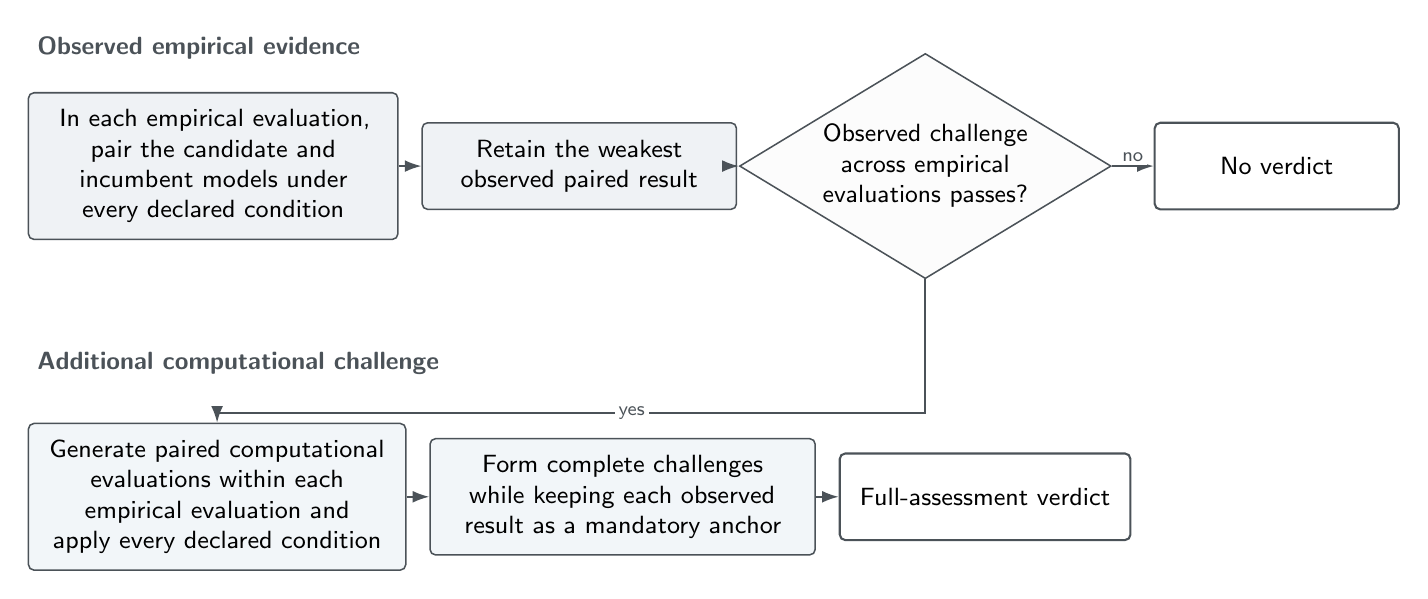
\begin{tikzpicture}[x=1mm,y=1mm]

  \node[stage] at (0,15) (stage1) {Observed empirical evidence};

  \node[observed,text width=42mm,anchor=west] at (0,0) (pair) {
    In each empirical evaluation, pair the candidate and incumbent models under every declared condition
  };

  \node[observed,text width=35mm,anchor=west] at (50,0) (anchor) {
    Retain the weakest observed paired result
  };

  \node[gate,anchor=center] at (114,0) (gate) {
    Observed challenge\\across empirical\\evaluations passes?
  };

  \node[endpoint,text width=21mm,anchor=west] at (143,0) (stop) {
    No verdict
  };

  \node[stage] at (0,-25) (stage2) {Additional computational challenge};

  \node[compute,text width=43mm,anchor=west] at (0,-42) (replicate) {
    Generate paired computational evaluations within each empirical evaluation and apply every declared condition
  };

  \node[compute,text width=44mm,anchor=west] at (51,-42) (anchored) {
    Form complete challenges while keeping each observed result as a mandatory anchor
  };

  \node[endpoint,text width=32mm,anchor=west] at (103,-42) (full) {
    Full-assessment verdict
  };

  \draw[arrow] (pair) -- (anchor);
  \draw[arrow] (anchor) -- (gate);
  \draw[arrow] (gate) -- node[branch,above] {no} (stop);
  \draw[arrow] (gate.south) -- ++(0,-17) -| node[branch,pos=0.22,right] {yes} (replicate.north);
  \draw[arrow] (replicate) -- (anchored);
  \draw[arrow] (anchored) -- (full);

\end{tikzpicture}
\end{document}
